% Numeric source: paper/shared/evidence/raw/iclr_model_behavior/analysis_v1/results.json
\section{Introduction}

A scene's floor plan can stay fixed while an embodied model's decisions change.
Converting materials alters color, contrast, and reflections without moving the
objects that define the task. A navigation instruction still refers to the same
destination, and a grounding query still refers to the same object. What changes
is the evidence the model sees. Material sensitivity asks whether the model
maintains the same task-relevant judgment across this appearance change. As simulated scenes move between rendering
systems, this seemingly technical asset operation becomes an experiment on
visual dependence.

\begin{figure}[t]
\centering
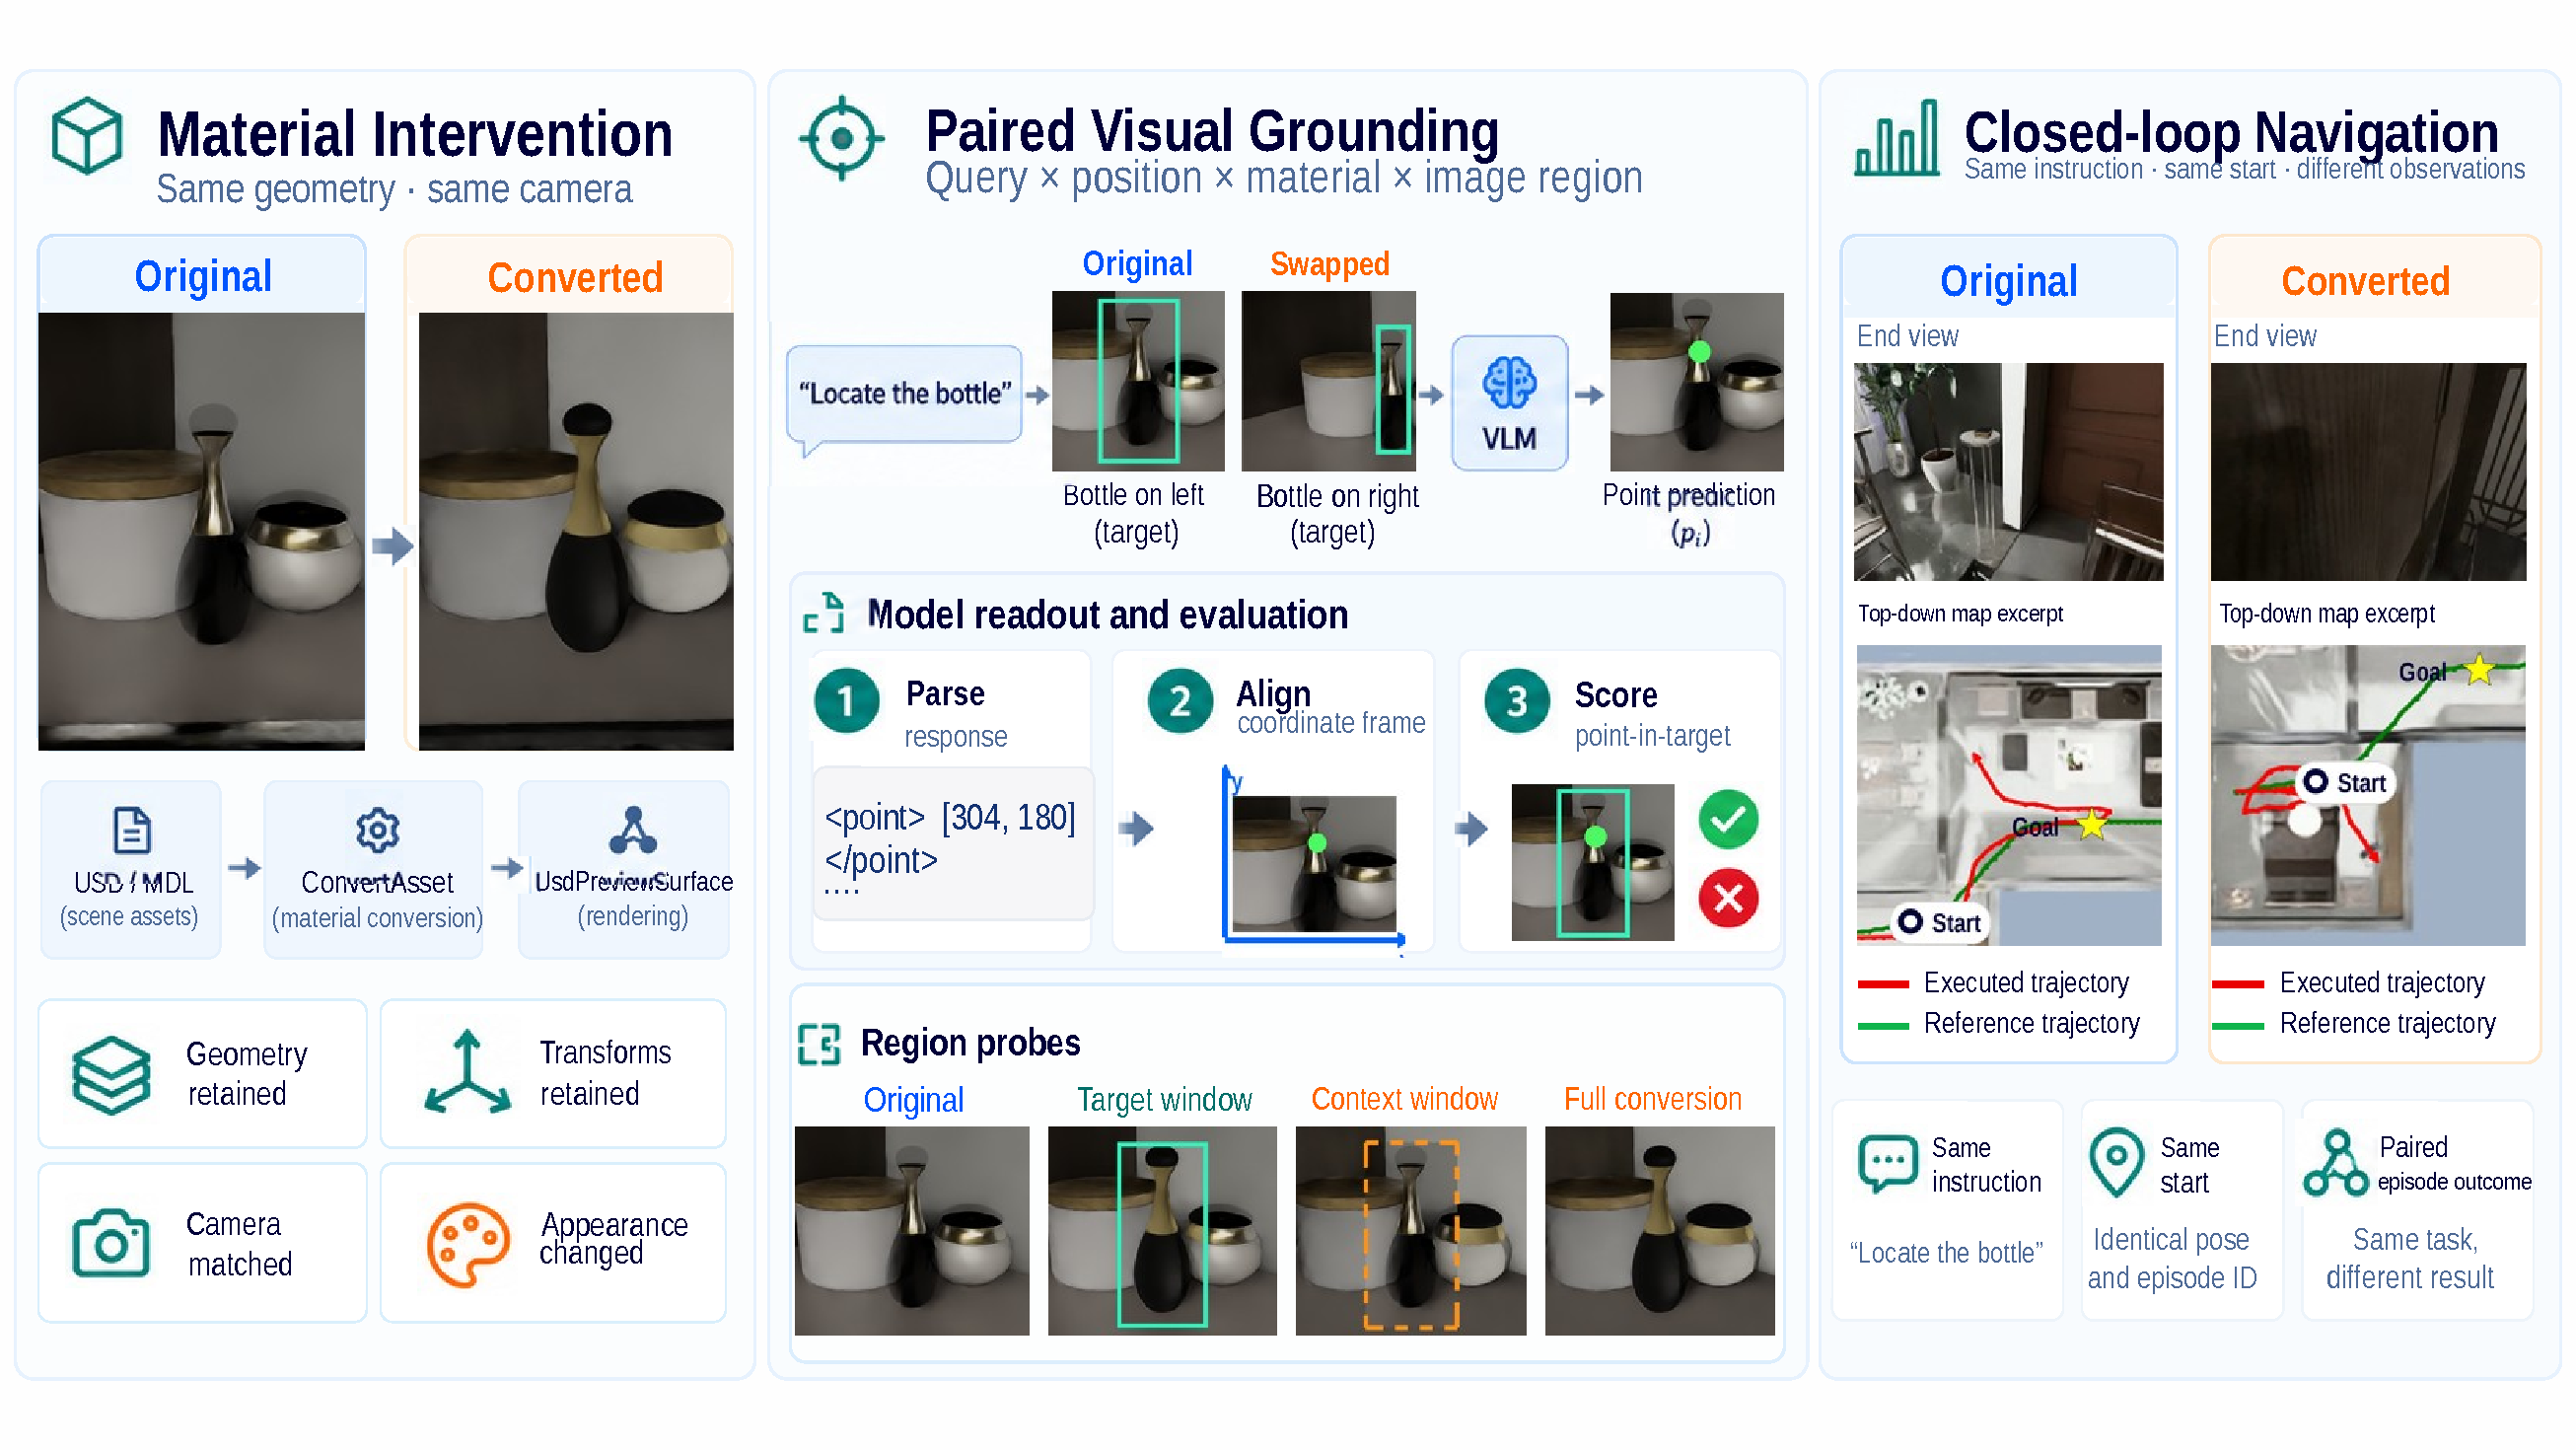
\includegraphics[width=\linewidth]{system_hero.pdf}
\caption{Probing material sensitivity in embodied models with ConvertAsset.
\emph{Left}: material conversion (USD/MDL $\rightarrow$ UsdPreviewSurface)
retains scene geometry, transforms, and camera while changing rendered
appearance. \emph{Middle}: paired visual grounding varies the query, the
target position, the material, and the image region; a parse--align--score
readout turns the recorded VLM point prediction into a point-in-target
decision, and region probes isolate where appearance changes matter.
\emph{Right}: closed-loop navigation pairs episodes that share the
instruction, the start pose, and the episode ID but differ in observations.
All image panels show recorded model inputs, recorded predictions, and
recorded navigation runs.}
\label{fig:system}
\end{figure}

The consequences are easy to miss in aggregate. In our paired navigation
evaluation, success falls from \NavSrOriginal\% to \NavSrConverted\%, but
\NavFlipPercent\% of episodes change success status. Seventeen previously
successful episodes fail; thirteen previously failed episodes succeed. A net
loss of four thus hides thirty changed outcomes. Mean accuracy describes how
many tasks succeed, but loses track of which tasks succeed.

Visual grounding brings this question into sharper focus. Given paired images,
we can ask whether a model still points to the requested object, then change
the query, the object's position, or only part of the image. A point prediction
also introduces an important measurement problem: the same response can map to
different locations under different coordinate conventions. We therefore
separate the model's visual dependence from the interface used to express a
location before interpreting its response to material conversion.

\begin{figure}[t]
\centering
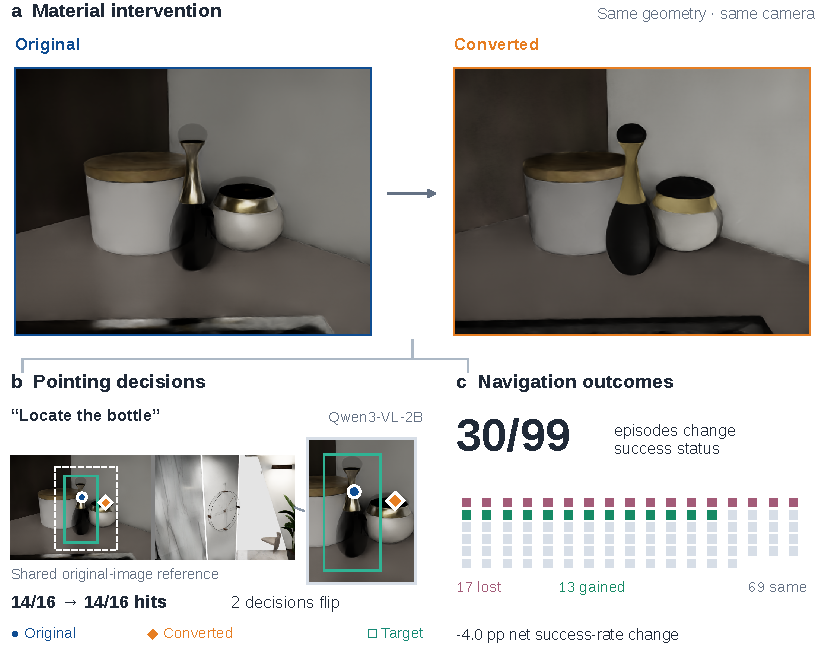
\includegraphics[width=\linewidth]{overview.pdf}
\caption{Same scene, different decisions. (a) Original MDL and converted
UsdPreviewSurface views retain scene geometry. (b) Grounding points from both
conditions share an original-image reference; the dashed outline identifies
the enlargement and the green box marks the target. Neither outline is shown
to the model. Equal hit totals hide changes in which queries succeed.
(c) Navigation has 30 changed outcomes but a net loss of four successes.}
\label{fig:overview}
\end{figure}

We start from USD scenes with NVIDIA MDL materials and construct UsdPreviewSurface
counterparts while preserving scene composition and geometry.
Figure~\ref{fig:system} organizes these paired interventions;
Figure~\ref{fig:overview} previews the resulting changes in model decisions. A readout experiment spans six
vision-language model (VLM) configurations. Controlled two-view experiments then
make the query determine the target: two objects share a canvas, their positions
are swapped, and the image center lies between them. Finally, region crossovers
replace the target window or its context to ask where appearance changes matter.
In a separate navigation evaluation, the material intervention changes the
observations available throughout an episode.

The experiments establish three connected findings. Spatial readout can reshape
the measured material effect; target and context changes can push grounding in
opposite directions; and small net navigation changes can conceal substantial
turnover in successful episodes. Together, they characterize material
sensitivity at the level of paired decisions, from a single point to an episode
outcome. This perspective makes the identity of successful queries and episodes
part of the evaluation, alongside their total number.
The accompanying experimental package preserves the inputs, responses, and
pairing needed to trace those changes.
